\documentclass{article}
\usepackage{tikz}
\usetikzlibrary{arrows.meta}
\begin{document}
% 箭头符号
% 在路径的起始或结束位置使用箭头,需要使用arrows.meta库,参考section 16
%   1)arrows={[<start_arrow>]-[<end_arrow>]}
%     在路径起始和结束处放置箭头,路径不能为闭合线条
%     省略start_arrow或end_arrow时,不显示该箭头
%     arrows参数名也可省略
%   2)箭头类型:
%   小写字母开头为老版本兼容,不可带参数;大写字母开头为新版本,可带参数进行箭头调整
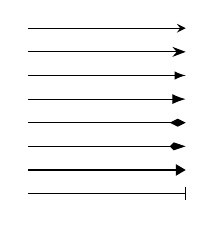
\begin{tikzpicture}
    \draw[-stealth] (0,-0.3) -- ++(2,0);
    \draw[-Stealth] (0,-0.6) -- ++(2,0);
    \draw[-latex] (0,-0.9) -- ++(2,0);
    \draw[-Latex] (0,-1.2) -- ++(2,0);
    \draw[-Diamond] (0,-1.5) -- ++(2,0);
    \draw[-Kite] (0,-1.8) -- ++(2,0);
    \draw[-Triangle] (0,-2.1) -- ++(2,0);
    \draw[-Bar] (0,-2.4) -- ++(2,0);
\end{tikzpicture}


%   3)设置箭头属性{<arrow>[<attributes>]}. 属性列表:
%     [1]length=<dimension> [<line_width_factor>] [<outer_factor>]
%       箭头的顶部和尾部的距离长度. 参数列表如下:
%         dimension - 箭头的长度
%         line_width_factor - 如果指定该值,则箭头长度 = dimension + line_width_factor * line_width
%         outer_factor - 适用于双边框线的情况. w_i为细线宽度(double distance),w_o为单侧外线宽度(line width),w_t为粗线宽度
%           w = out_factor * w_o + (1 - out_factor) * w_t
%           将w作为line_width_factor参数公式里的line_width
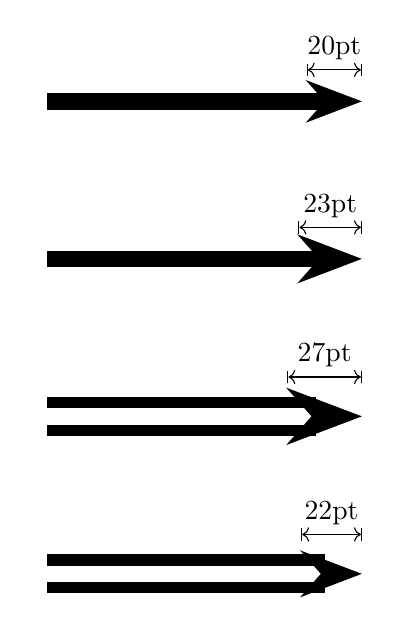
\begin{tikzpicture}{>=stealth}
    \draw[line width=6pt,-{Stealth[length=20pt]}] (0,0) -- ++(4,0);
    \draw[|<->|] (4cm-20pt,0.4) -- ++(20pt,0) node[pos=0.5,above]{20pt};

    \draw[line width=6pt,-{Stealth[length=20pt 0.5]}] (0,-2) -- ++(4,0);
    \draw[|<->|] (4cm-23pt,-2+0.4) -- ++(23pt,0) node[pos=0.5,above]{23pt};

    \draw[line width=4pt,double,double distance=6pt,-{Stealth[length=20pt 0.5 0]}] (0,-4) -- ++(4,0);
    \draw[|<->|] (4cm-27pt,-4+0.5) -- ++(27pt,0) node[pos=0.5,above]{27pt};

    \draw[line width=4pt,double,double distance=6pt,-{Stealth[length=20pt 0.5 1]}] (0,-6) -- ++(4,0);
    \draw[|<->|] (4cm-22pt,-6+0.5) -- ++(22pt,0) node[pos=0.5,above]{22pt};
\end{tikzpicture}

%     [2]width=<dimension> [<line_width_factor>] [<outer_factor>]
%       箭头的上侧与下侧的距离长度. 参数列表如下:
%         dimension - 箭头的宽度
%         line_width_factor - 如果指定该值,则箭头宽度 = dimension + line_width_factor * line_width
%         outer_factor - 适用于双边框线的情况. w_i为细线宽度,w_o为单侧外线宽度,w_t为粗线宽度
%           w = out_factor * w_o + (1-out_factor) * w_t
%           将w作为line_width_factor参数公式里的line_width
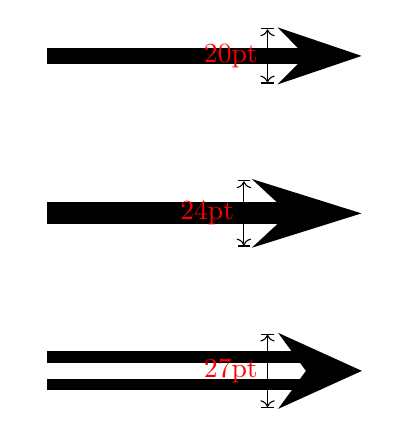
\begin{tikzpicture}{>=stealth}
    \draw[line width=6pt,-{Stealth[width=20pt]}] (0,0) -- ++(4,0);
    \draw[|<->|] (2.8,-10pt) -- ++(0,20pt) node[pos=0.5,left]{\color{red}20pt};

    \draw[line width=8pt,-{Stealth[width=20pt 0.5]}] (0,-2) -- ++(4,0);
    \draw[|<->|] (2.5,-2cm-12pt) -- ++(0,24pt) node[pos=0.5,left]{\color{red}24pt};

    \draw[line width=4pt,double,double distance=6pt,-{Stealth[width=20pt 0.5 0]}] (0,-4) -- ++(4,0);
    \draw[|<->|] (2.8,-4cm-13.5pt) -- ++(0,27pt) node[pos=0.5,left]{\color{red}27pt};
\end{tikzpicture}

%     [3]width'=<dimension> [<length_factor>] [<line_width_factor>]
%       箭头的上侧与下侧的距离长度,类似于width. width = dimension + length_factor * arrow_length + line_width_factor * line_width

%     [4]inset=<dimension> [<line_width_factor>] [<outer_factor>]
%       箭头尾部凹进去的距离长度(只对部分箭头有效). 参数列表如下:
%         dimension - 凹进去的长度
%         line_width_factor - 如果指定该值,则内凹长度 = dimension + line_width_factor * line_width
%         outer_factor - 适用于双边框线的情况. w_i为细线宽度,w_o为单侧外线宽度,w_t为粗线宽度
%           w = out_factor * w_o + (1-out_factor) * w_t
%           将w作为line_width_factor参数公式里的line_width
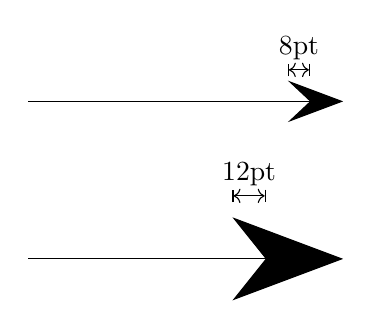
\begin{tikzpicture}{>=stealth}
    \draw[-{Stealth[length=20pt,inset=8pt]}] (0,0) -- ++(4,0);
    \draw[|<->|] (4cm-20pt,0.4) -- ++(8pt,0) node[pos=0.5,above]{8pt};

    \draw[-{Stealth[length=40pt,inset=12pt]}] (0,-2) -- ++(4,0);
    \draw[|<->|] (4cm-40pt,-2+0.8) -- ++(12pt,0) node[pos=0.5,above]{12pt};
\end{tikzpicture}

%     [5]inset'=<dimension> [<length_factor>] [<line_width_factor>]
%       箭头内凹的距离长度,类似于inset. inset = dimension + length_factor * arrow_length + line_width_factor * line_width

%     [6]angle=<angle>:<dimension> [<line_width_factor>] [<outer_factor>]
%       同时设定箭头的长度和宽度. 参数列表如下:
%         angle - 箭头顶部角度. length = dimension * cos(1/2 * angle), width = 2 * dimension * sin(1/2 * angle)
%         line_width_factor - 如果指定该值,则dimension = dimension + line_width_factor * line_width
%         outer_factor - 适用于双边框线的情况. w_i为细线宽度,w_o为单侧外线宽度,w_t为粗线宽度
%           w = out_factor * w_o + (1-out_factor) * w_t
%           将w作为line_width_factor参数公式里的line_width
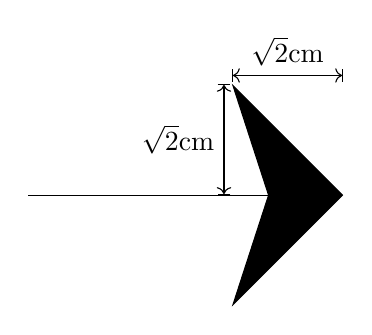
\begin{tikzpicture}{>=stealth}
    \draw[-{Stealth[angle=90:2cm]}] (0,0) -- ++(4,0);
    \draw[|<->|] ({4-sqrt(2)},1.52) -- ++({sqrt(2)},0) node[pos=0.5,above]{$\sqrt{2}$cm};
    \draw[|<->|] ({4-sqrt(2)-0.1},0) -- ++(0,{sqrt(2)}) node[pos=0.5,left]{$\sqrt{2}$cm};
\end{tikzpicture}

%     [7]angle'=<angle>
%       设置箭头的宽度. width = 2 * length * tan(1/2 * angle)

%     [8]scale=<factor> 
%       箭头伸缩系数
%     [9]scale length=<factor>
%        scale width=<factor>
%       箭头长度或宽度伸缩系数

%     [10]slant=<factor>
%       箭头倾斜值. cot(angle), angle为坡度角
\begin{tikzpicture}{>=stealth}
    \draw[-{Bar[slant=0.5]}] (0,0) -- ++(4,0);
    \draw[-{Bar[slant=1]}] (0,-2) -- ++(4,0);
    \draw[-{Bar[slant=2]}] (0,-4) -- ++(4,0);
\end{tikzpicture}

%     [11]reversed
%       箭头方向进行翻转
\begin{tikzpicture}{>=stealth}
    \draw[-{Stealth}] (0,0) -- ++(4,0);
    \draw[-{Stealth[reversed]}] (0,-4) -- ++(4,0);
\end{tikzpicture}

%     [12]harpoon - 只保留沿着箭头方向的左侧
%     [13]swap - 沿着箭头方向进行折叠,配合harpoon使用,只保留沿着箭头方向的右侧
%     [14]left/right - left类似于harpoon,right类似于harpoon和swap组合
\begin{tikzpicture}{>=stealth}
    \draw[-{Stealth[harpoon]}] (0,0) -- ++(4,0);
    \draw[-{Stealth[harpoon,swap]}] (0,-1) -- ++(4,0);
\end{tikzpicture}

%     [15]color - 箭头边框和填充颜色
%     [16]fill - 箭头的填充颜色
%     [17]open - 箭头填充处为透明,类似于fill=none
\begin{tikzpicture}{>=Stealth}
    \draw[-{Stealth[color=red]}] (0,0) -- ++(4,0);
    \draw[-{Stealth[color=red,fill=blue]}] (0,-1) -- ++(4,0);
    \fill[blue!30] (4,-2) circle [radius=5pt];
    \draw[-{Stealth[open]}] (0,-2) -- ++(4,0);
\end{tikzpicture}

%     [18]line cap
%       端点尖锐或圆滑. butt/round
%     [19]line join
%       箭头顶部交点处尖锐或圆滑. round/miter
%     [20]round - 类似于line cap=round,line join=round
%     [21]sharp - 类似于line cap=butt,line join=miter

%     [22]line width=<dimension> [<line_width_factor>] [<outer_factor>]
%       箭头的线条宽度. 参数列表如下:
%         dimension - 线条的宽度
%         line_width_factor - 如果指定该值,则箭头线条宽度 = dimension + line_width_factor * line_width
%         outer_factor - 适用于双边框线的情况. w_i为细线宽度,w_o为单侧外线宽度,w_t为粗线宽度
%           w = out_factor * w_o + (1-out_factor) * w_t
%           将w作为line_width_factor参数公式里的line_width
%     [23]line width'=<dimension> [<length_factor>]
%       箭头的线条宽度. 参数列表如下:
%         dimension - 线条的宽度
%         length_factor - 如果指定该值,则箭头线条宽度 = dimension + length_factor * length

%     [24]quick
%       箭头尾部,在箭头头部点所在线条的切线上. 默认箭头尾部位置确认方式
%       该方式适用于直线,不适用于曲线
%     [25]flex=<factor>
%       箭头尾部,确保在path路径上. 需要导入bending tikz库,导入bending后的默认项
%       该方式适用于曲线,计算复杂度高于quick,不建议用于直线
%       factor - 为0时,与quick一致;为1代表完全依照path路径
%     [25]flex'=<factor>
%       箭头尾部方向,确保在与path路径方向一致. 需要导入bending tikz库
%       该方式适用于曲线,计算复杂度高于quick,不建议用于直线
%       factor' - 为0时,与quick一致;为1代表完全依照path路径
%     [26]bend
%       箭头弯曲以适应曲线. 需要导入bending tikz库
%       该方式适用于曲线,计算复杂度高于flex/flex',不建议用于直线
\begin{tikzpicture}{>=Stealth}
    \wall
    \draw [red!25,line width=1mm] (-1,0) -- (1,0);
    \draw [red,line width=1mm,-{Stealth[length=1cm,open,blue,quick]}] (-1,-.5) .. controls (0,-.5) and (0,0) .. (1,0);
    \begin{scope}[yshift=-2cm]
        \wall
        \draw [red!25,line width=1mm] (-1,0) -- (1,0);
        \draw [red,line width=1mm,-{Stealth[length=1cm,open,blue,flex]}] (-1,-.5) .. controls (0,-.5) and (0,0) .. (1,0);
    \end{scope}
    \begin{scope}[yshift=-4cm]
        \wall
        \draw [red!25,line width=1mm] (-1,0) -- (1,0);
        \draw [red,line width=1mm,-{Stealth[length=1cm,open,blue,flex']}] (-1,-.5) .. controls (0,-.5) and (0,0) .. (1,0);
    \end{scope}
    \begin{scope}[yshift=-6cm]
        \wall
        \draw [red!25,line width=1mm] (-1,0) -- (1,0);
        \draw [red,line width=1mm,-{Stealth[length=1cm,open,blue,bend]}] (-1,-.5) .. controls (0,-.5) and (0,0) .. (1,0);
    \end{scope}
\end{tikzpicture}


%   4)配置默认箭头'>='
\begin{tikzpicture}[>=stealth]
    \draw[->] (0,0) -- (2,0);
\end{tikzpicture}


%   5)端点多箭头
\begin{tikzpicture}
    \draw[-{Stealth[] Bar[scale=6]}] (-2,0) -- (2,0);
\end{tikzpicture}


%   6)箭头后保留一定空格
%     sep=<dimension> [<line_width_factor>] [<outer_factor>]
%       箭头后保留空格长度,默认为0.88pt .3 1. 参数列表如下:
%         dimension - 空格的长度
%         line_width_factor - 如果指定该值,则空格长度 = dimension + line_width_factor * line_width
%         outer_factor - 适用于双边框线的情况. w_i为细线宽度,w_o为单侧外线宽度,w_t为粗线宽度
%           w = out_factor * w_o + (1-out_factor) * w_t
%           将w作为line_width_factor参数公式里的line_width


%   7)箭头之间是否作path
%     .
%     在起始端,.之前的箭头之间不作path;在结束段,.之后的箭头之间不作path
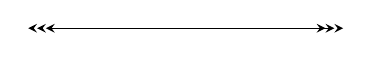
\begin{tikzpicture}[>=stealth]
    \draw[<<.<->>.>] (-2,0) -- (2,0);
\end{tikzpicture}


%   8)定义箭头组的缩写
%     <key>/.tip=<arrow_spec>
\begin{tikzpicture}[mine/.tip={Latex[red,sep] Stealth[blue]}]
    \draw[-mine] (-2,0) -- (2,0);
\end{tikzpicture}

\end{document}
